% or aspectratio=43, +handout
\documentclass[aspectratio=169,handout]{beamer}

% remove this line for an english presentation
%\usepackage{ngerman}

% Optional arguments (separate by comma):
% darkmode			- Black background and white font
% imagetitlepage	- Adds the images defined in \titlegraphic to the title page
\usepackage[imagetitlepage]{lgdv/lgdv_beamer}

\usepackage{siunitx}
\usepackage{mdframed}
\usepackage{pgfplots}
\usepackage{filecontents}
\usepackage{tikz}
\usepackage{xcolor}
\graphicspath{{images/}}


%make existing function names bold
\lstset%
{%
	%
	% Custom Types for Syntax Highlighting
	%
	emph=[0]%
	{%
		Particle,PositionRadius,VelocityMass
	},
	emphstyle=[0]{\bfseries\color{typecolor}},
}



\subtitle{AGPhys WS 20/21}
\title{Hardware Architecture and Parallel Communication}
\author[Darius Rückert]{Darius Rückert}
\date{\today}

\titlegraphic
{
	\begin{figure}[!h]
	
\includegraphics[height=.4\textheight]{cuda}
	\hfil
	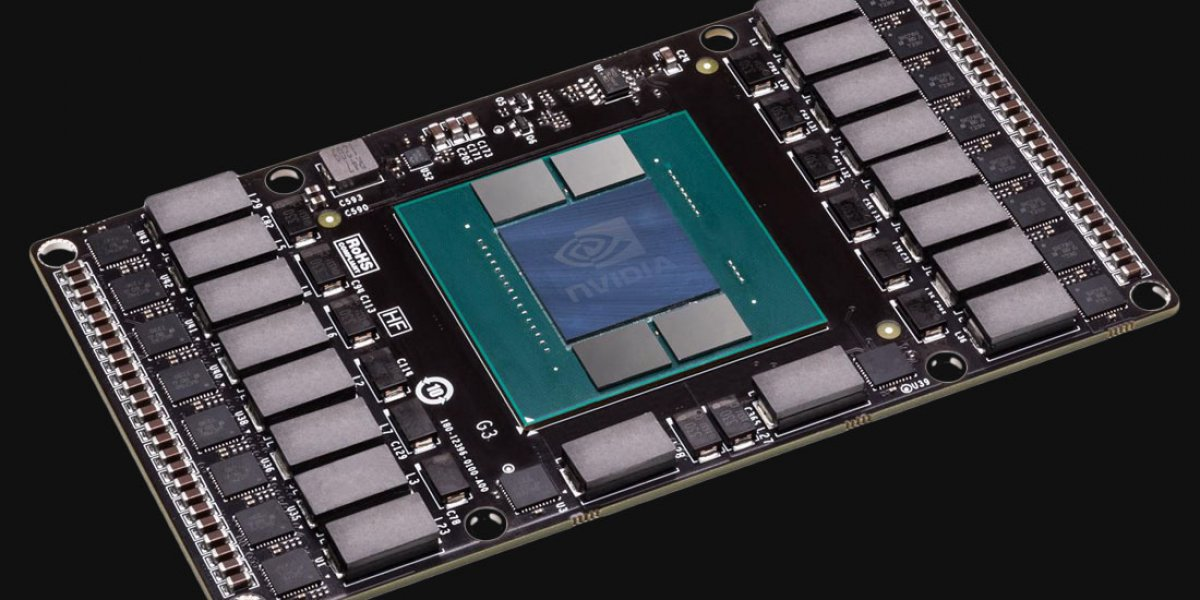
\includegraphics[height=.4\textheight]{ddr5}
	\hfil
	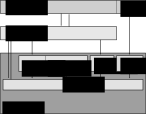
\includegraphics[height=.4\textheight]{globalMemory}
	\end{figure}
}

\begin{document}

\frame
{
	\titlepage
}


\begin{frame}[fragile]
	\frametitle{Blocks and Warps}
	From last lecture we have learned...
	\begin{itemize}
		\item Kernels are launched on blocks of threads
		\item A threadblock is executed in Warps of 32 threads
		\item [$\rightarrow$] This matches the hierarchical architecture of GPUs
	\end{itemize}
\end{frame}

\frame
{
	\frametitle{GPU Architecture}
	\begin{figure}
		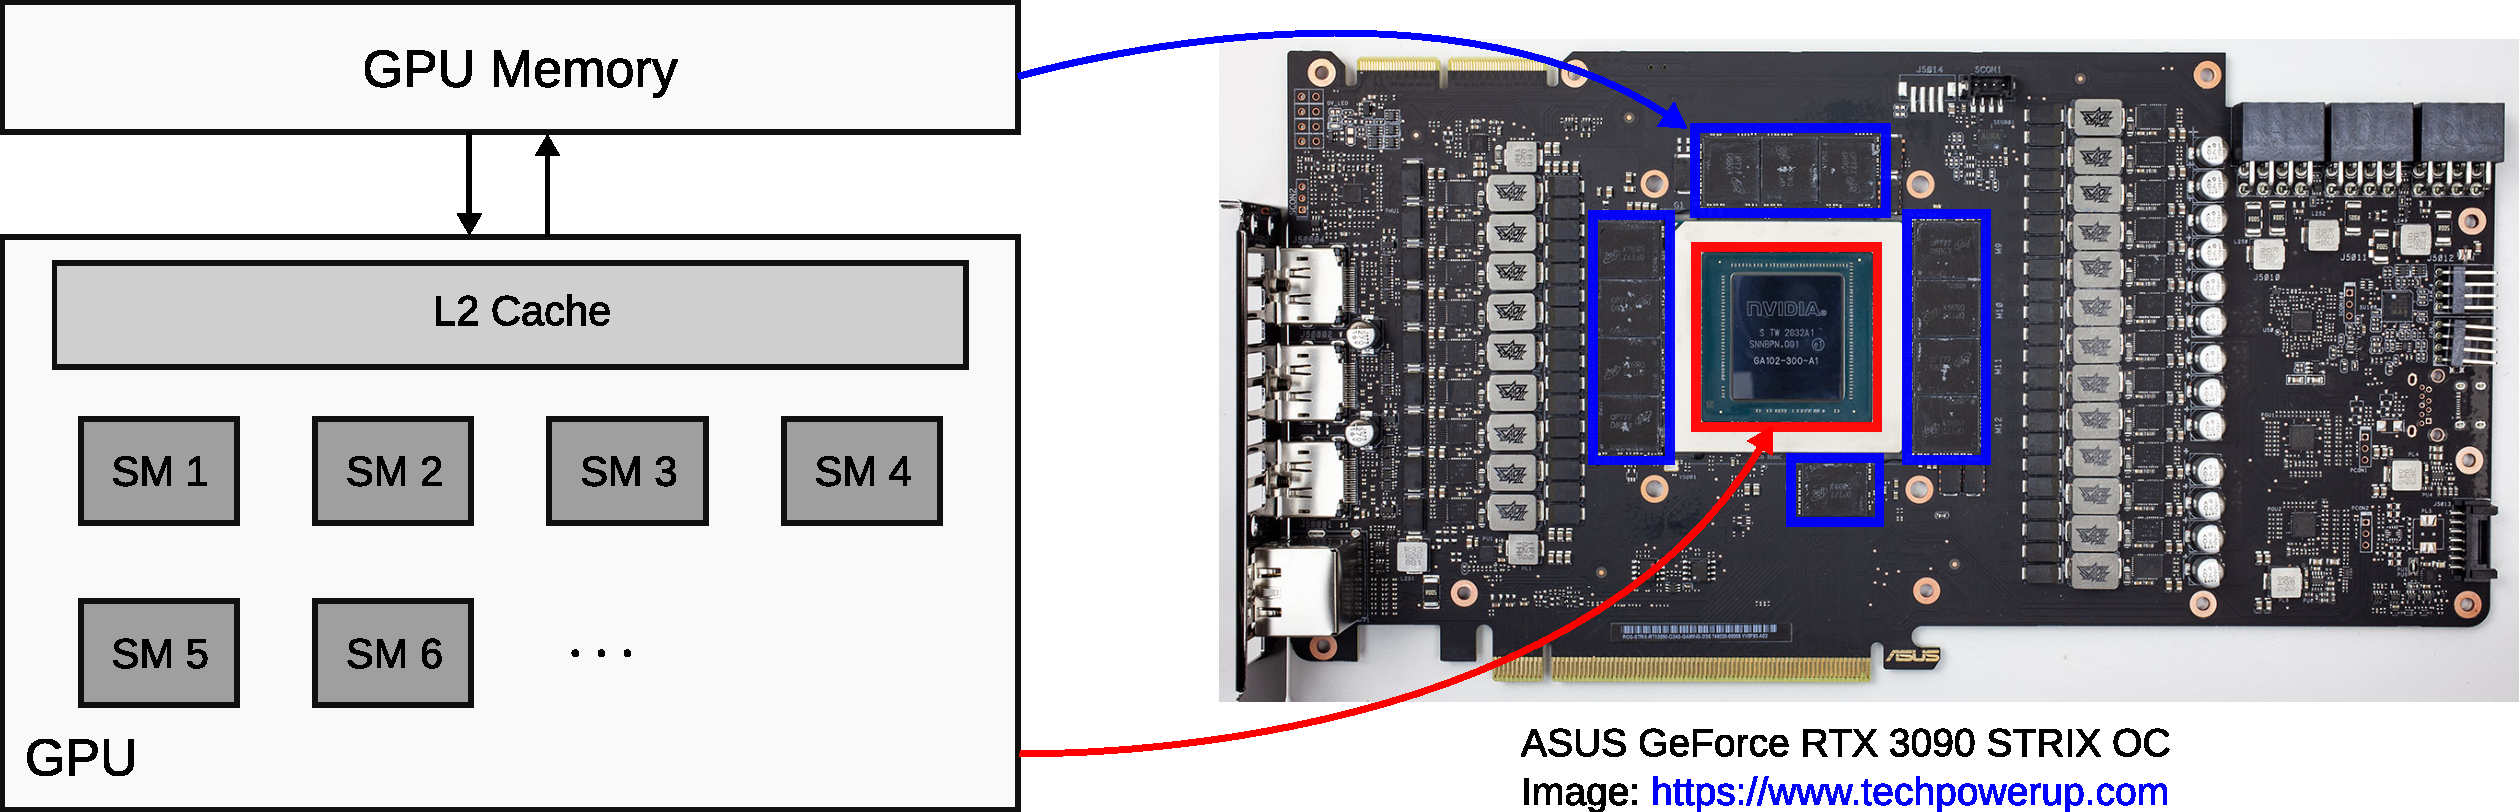
\includegraphics[width=1.0\textwidth]{arch}
	\end{figure}
}

\begin{frame}[fragile]
	\frametitle{Streaming Multiprocessor (SM)}
	A GPU consists of multiple streaming multiprocessors (SM)
	\begin{itemize}
		\item GTX 1080 Ti: 28 SMs
		\item RTX 2080 Ti: 68 SMs
		\item RTX 3090: 82 SMs
	\end{itemize}
	The \textbf{scheduler} distributes \textbf{threadblocks} to the SMs
		\begin{itemize}
			\item Once scheduled, a threadblock runs till completion (no swap-out)
		\end{itemize}
\end{frame}


\frame
{
	\frametitle{Streaming Multiprocessor}
	\begin{minipage}{0.3\linewidth}
	\begin{figure}
		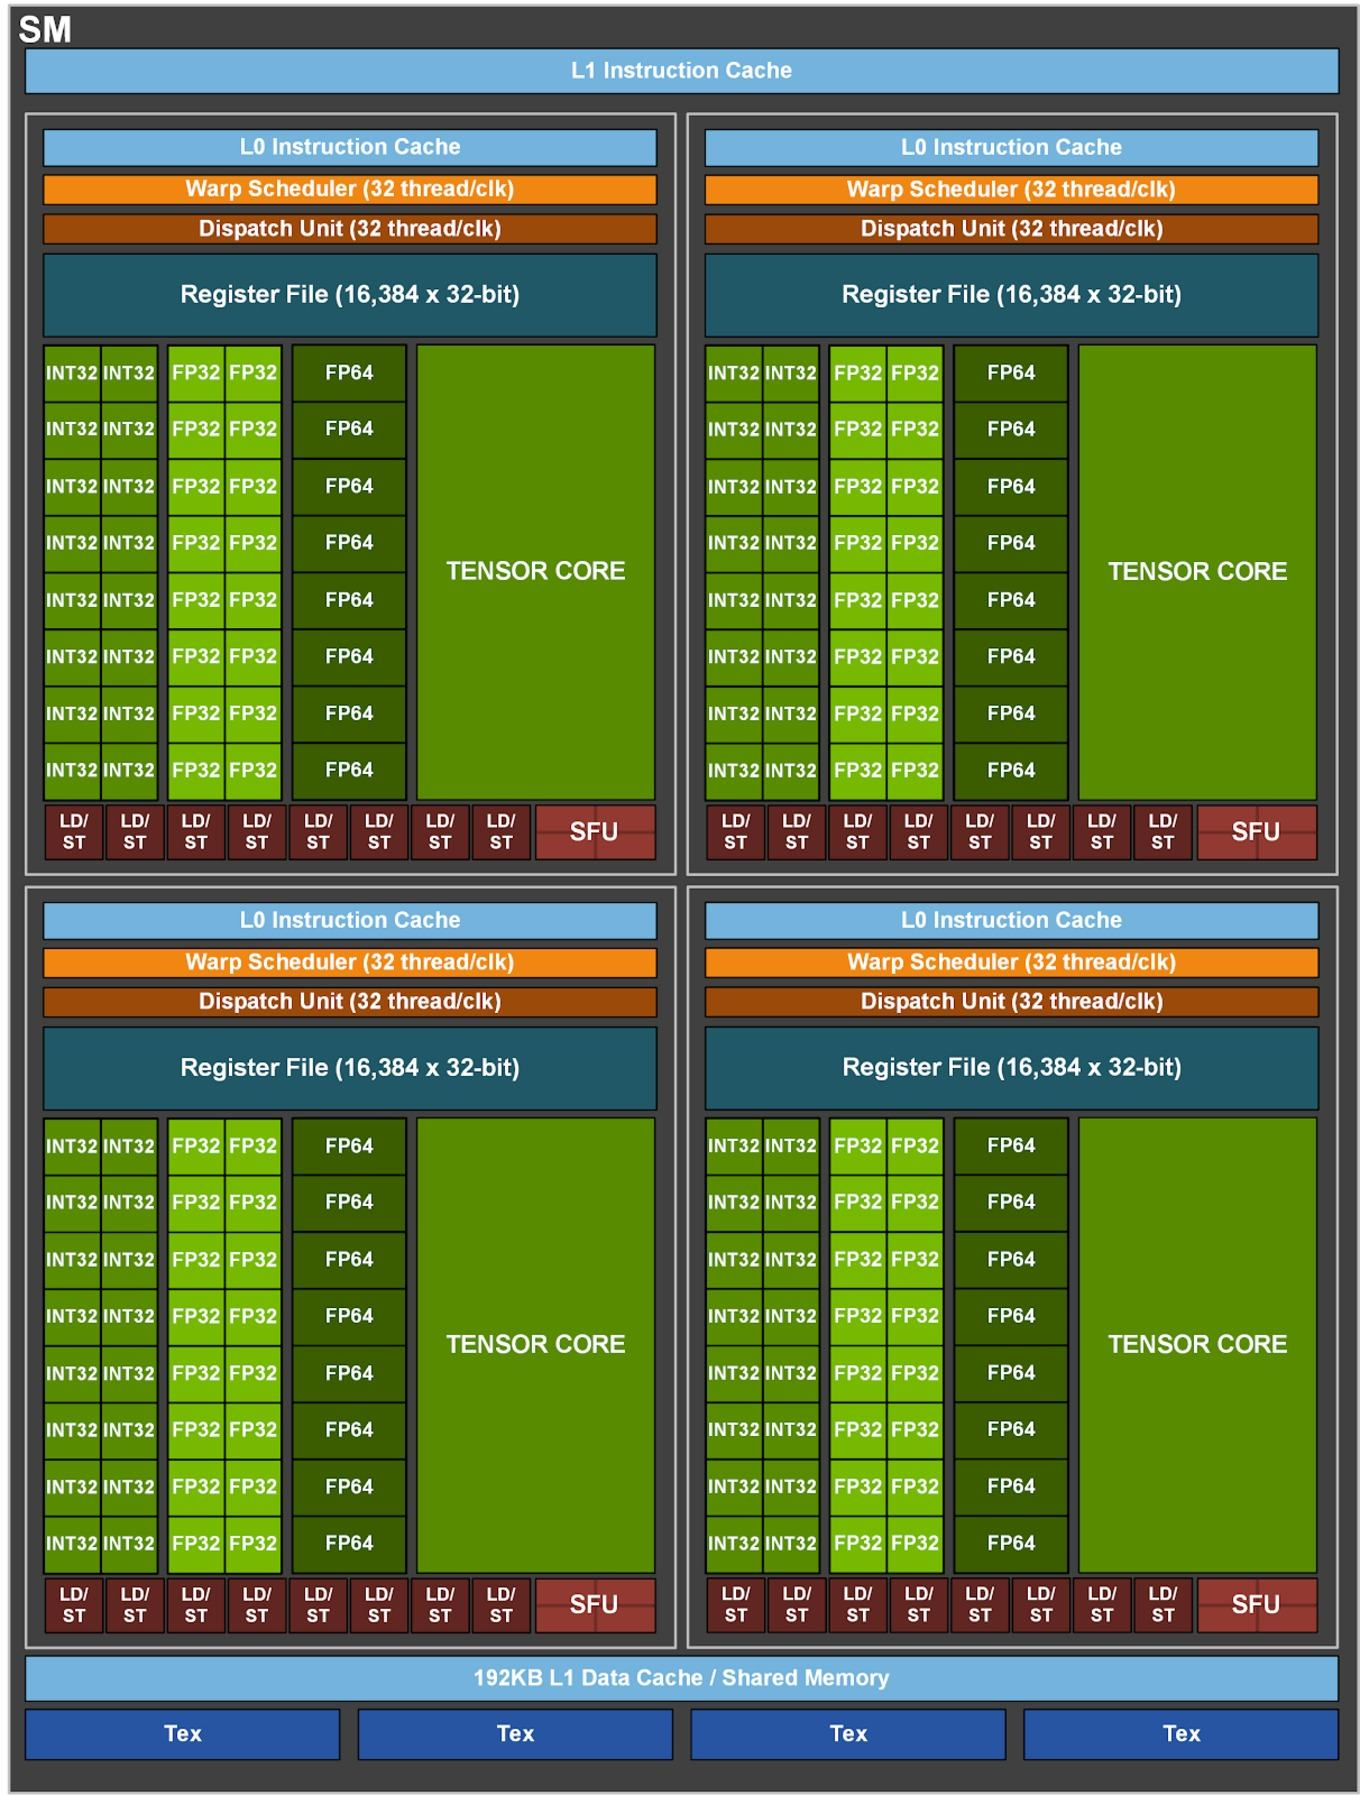
\includegraphics[height=0.8\textheight]{ampere_sm}
	\end{figure}
	\centering
	NVIDIA Ampere SM
	\end{minipage}
	\begin{minipage}{0.68\linewidth}
\begin{itemize}
	\item A SM can execute 4 Warps simultaneously
	\item $4 \cdot 32 = 128$ Threads
	\item[$\rightarrow$] 128 is often the best block size
	\item Each SM has an additional L1 Data Cache / Shared Memory
	\item The registers are shared for each Warp
	\item[$\rightarrow$] Threads in the same Warp can share variables over registers (shuffle)
\end{itemize}
	\end{minipage}
	
}





\frame
{
	\frametitle{Memory Access and Caches}
	\begin{minipage}{0.45\linewidth}
	\begin{figure}
		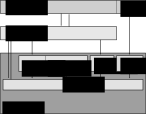
\includegraphics[height=0.8\textheight]{globalMemory}
	\end{figure}
	\end{minipage}
	\begin{minipage}{0.5\linewidth}
\begin{itemize}
	\item All global memory read and writes are cached in the L2 cache.
	\item<2-> Memory transactions through registers (load-store architecture)
	\item<3-> Optional L1 data cache on the SM
\end{itemize}
	\end{minipage}
	
}


\frame{
	\frametitle{Registers}
	\begin{itemize}
		\item Local variables are stored in registers (there is no stack!)
		\item The amount of registers is limited
	\end{itemize}
	\vspace{0.3cm}
 	If too many registers are used on a SM, either
	\begin{itemize}
		\item some variables are stored in global memory (slow)
		\item or the occupancy (number of running threads) is reduced (also slow)
	\end{itemize}	
	
		\vspace{0.3cm}
	\textbf{Note:} Local arrays are stored in registers if all accesses are compile time constant
}



\frame{
	\frametitle{Special Caches}
	The GPU memory can be accessed through various caches, optimized for different applications
	\\ \vspace{0.5cm}
	\begin{tabular}{l|l|l|l}
	Name & Location  & Optimal for &R/W\\	
	\hline
	L2 Data Cache  & Chip & &read/write \\
	L1 Data Cache  & SM   & random access & read-only\\
	Constant Cache & SM    & broadcast-reads & read-only \\
	Texture Cache  & SM    & spatial-reads & read-only \\
\end{tabular}
\\ \vspace{0.5cm}
\textbf{Note:} L1, Constant, and Texture Cache are not used by default! We need explicit setup/instructions for them.
}


\begin{frame}[fragile]
	\frametitle{L1 Cache}
	The L1 Cache can be used by defining a pointer to global memory as
\begin{lstlisting}
const __restrict__
\end{lstlisting}

	\textbf{Example Kernel:}
	\begin{lstlisting}
__global__ static
void crload(const int* __restrict__ data, int* result)
{
	result[threadIdx.x] = data[threadIdx.x] + 42;
}
	\end{lstlisting}
\end{frame}


\begin{frame}[fragile]
\frametitle{Random Memory Access}
\begin{figure}[!h]
	\begin{tikzpicture}
	\begin{axis}[
	xmode=log,
	log basis x={2},
	width=0.7\textwidth,height=0.5\textwidth,
	%axis equal,
	legend pos=north east,			
	xmin=1,
	domain=0:5,
	xlabel=Array Size (KiB),
	ylabel=Bandwidth (GB/s),
	ymin=0,ymax=450,
	%xmin=-0.5,xmax=0.5,ymin=-0.3,ymax=0.3,
	]
	%\addplot+[mark=none, color=black] table [x=x, y=y, col sep=comma] {images/0003.csv};
		\addplot+[mark=none] table [x=size, y=ldg, col sep=comma] {images/out.csv};
	\addplot+[mark=none] table [x=size, y=simple, col sep=comma] {images/out.csv};
	%\addplot+[mark=none] table [x=size, y=texture, col sep=comma] {images/out.csv};

	\addlegendentry{With L1}
	\addlegendentry{Without L1}
	
	\end{axis}
	\end{tikzpicture}
\end{figure}
\end{frame}


\begin{frame}[fragile]
	\frametitle{Constant Cache, Constant Memory}
	\begin{itemize}
		\item Is specialized for \textbf{broadcast-reads}
		\begin{itemize}
			\item All threads in a warp access the same element
		\end{itemize}
		\item Non-broadcast reads are serialized!
	\end{itemize}
	To use the constant cache, the data has to be placed in \textbf{constant memory}.
	\begin{lstlisting}
	// Global array in constant memory (accessible from all kernels)
	static __constant__ int cweights[1024];

	// Host code to initialize constant memory
	thrust::host_vector<int> weight(1024,5);
	cudaMemcpyToSymbol(cweights,weight.data().get(),weight.size() * 	   sizeof(int),cudaMemcpyHostToDevice);
	\end{lstlisting}
	

\end{frame}

\begin{frame}[fragile]
\frametitle{Texture Memory, Texture Cache}
	\begin{itemize}
		\item Is specialized for \textbf{2D spatial reads}
		\item Enables hardware interpolation, clamping 
	\end{itemize}
	Basic Usage:
\begin{enumerate}
	\item Create a CUDA texture object
	\item Bind the memory to the texture object
	\item Use the texture in a kernel
\end{enumerate}
\vspace{0.2cm}
More information: \url{https://docs.nvidia.com/cuda/cuda-c-programming-guide/index.html#texture-memory}
\end{frame}



\begin{frame}[fragile]
%\frametitle{Texture Memory, Texture Cache}
\begin{center}
\Large Synchronization and Communication
\end{center}
\end{frame}


\begin{frame}[fragile]
	\frametitle{Asynchronous Kernel Launches}
	\begin{minipage}{0.45\linewidth}
\begin{lstlisting}
// Asynchronous Kernel Launch
someKernel<<<5,128>>>(d_data);

// Do some CPU work
foo();

// Wait until all previous 
// kernels are finished and 
// copy the data
cudaMemcpy(h_data,d_data,size,cudaMemcpyDeviceToHost);
\end{lstlisting}
	\end{minipage}
	\begin{minipage}{0.5\linewidth}
\begin{itemize}
	\item<2-> CUDA Kernel launches are asynchronous
	\item<3->[$\rightarrow$] The control returns immediately to the CPU thread
	\item<4-> Some CUDA API functions are synchronous
	\item<5->[$\rightarrow$] The CPU waits for completion
\end{itemize}
	\end{minipage}
\end{frame}


\begin{frame}[fragile]
\frametitle{Asynchronous Kernel Launches}
\begin{minipage}{0.45\linewidth}
\begin{lstlisting}
// Asynchronous Kernel Launch
someKernel<<<5,128>>>(d_data);

// Do some CPU work
foo();

// Wait until all previous 
// kernels are finished and 
// copy the data
cudaMemcpy(h_data,d_data,size,cudaMemcpyDeviceToHost);
\end{lstlisting}
\end{minipage}
\begin{minipage}{0.5\linewidth}
	\vspace{0.3cm}
		\begin{figure}
	\includegraphics[height=0.9\textheight]{asynclaunch}
\end{figure}
\end{minipage}
\end{frame}



\begin{frame}[fragile]
\frametitle{Communication and Synchronization}
Threads communicate and are synchronized depending on their hierarchy level.
\begin{itemize}
		\item<1->[] \textbf{Between threads of different blocks}
	\begin{itemize}
		\item<2-> Communication via global memory
		\item<2-> No build-in synchronization primitives
	\end{itemize}
	\item<3->[] \textbf{Between threads of the same block}
\begin{itemize}
	\item<4-> Communication via shared memory
	\item<4-> Barrier synchronization with \texttt{\_\_syncthreads}
\end{itemize}
	\item<5->[] \textbf{Between threads of the same Warp}
	\begin{itemize}
		\item<6-> Communication via registers 
		\item<6-> Implicit synchronization (Pascal and earlier)
		\item<6-> Barrier synchronization with \texttt{\_\_syncwarp} (Volta, Turing, Ampere)

	\end{itemize}
\end{itemize}
\end{frame}




\begin{frame}[fragile]
\frametitle{Atomic Operations}
\begin{mdframed}[frametitle={CUDA Programming Guide}]
An atomic function performs a \textbf{read-modify-write atomic operation} on one 32-bit or 64-bit word residing in \textbf{global or shared memory}. For example, atomicAdd() reads a word at some address in global or shared memory, adds a number to it, and writes the result back to the same address. The operation is atomic in the sense that it is \textbf{guaranteed to be performed without interference from other threads}.
\end{mdframed}

\vspace{1cm}
\textbf{Note:} Atomic operations can be performed on global memory and shared memory.

\end{frame}


\begin{frame}[fragile]
\frametitle{Atomic Operations}

\textbf{atomicAdd/atomicSub}
\begin{itemize}
	\item Adds/subtracts \textit{val} to/from \textit{address}.
	\item Returns the old value of \textit{address}.
\begin{lstlisting}
T atomicAdd(T* address, T val);
\end{lstlisting}
\end{itemize}

\textbf{atomicMin/atomicMax}
\begin{itemize}
		\item Computes the maximum/minimum of \textit{val} and \textit{address}.
		\item Stores the result in \textit{address}.
		\item Returns the old value of \textit{address}.
\begin{lstlisting}
T atomicMin(T* address, T val);
\end{lstlisting}
\end{itemize}


\end{frame}

\begin{frame}[fragile]
\frametitle{Atomic Operations}

\textbf{atomicAnd/atomicOr/AtomicXor}
\begin{itemize}
	\item Computes bitwise and/or/xor of \textit{val} and \textit{address}.
	\item Stores the result in \textit{address}.
	\item Returns the old value of \textit{address}.
\begin{lstlisting}
T atomicAnd(T* address, T val);
\end{lstlisting}
\end{itemize}

\textbf{atomicInc/atomicDec}
\begin{itemize}
	\item Increments/Decrements \textit{address}.
	\item The result is moduloed by \textit{val}.
	\item Returns the old value of \textit{address}.
\begin{lstlisting}
T atomicInc(T* address, T val);
\end{lstlisting}
\end{itemize}
\end{frame}



\begin{frame}[fragile]
\frametitle{Atomic Operations}

\textbf{atomicExch}
\begin{itemize}
	\item Sets \textit{address} to \textit{val}
	\item Returns the old value of \textit{address}.
\begin{lstlisting}
T atomicExch(T* address, T val);
\end{lstlisting}
\end{itemize}

\textbf{atomicCAS}
\begin{itemize}
	\item Sets \textit{address} to \textit{val}, if \textit{address} is equal to \textit{compare}
	\item Returns the old value of \textit{address}.
\begin{lstlisting}
T atomicCAS(T* address, T compare, T val);
\end{lstlisting}
\end{itemize}
\end{frame}

\frame
{
	\frametitle{Example: Red-Blue Collision Detection}
	\begin{figure}
		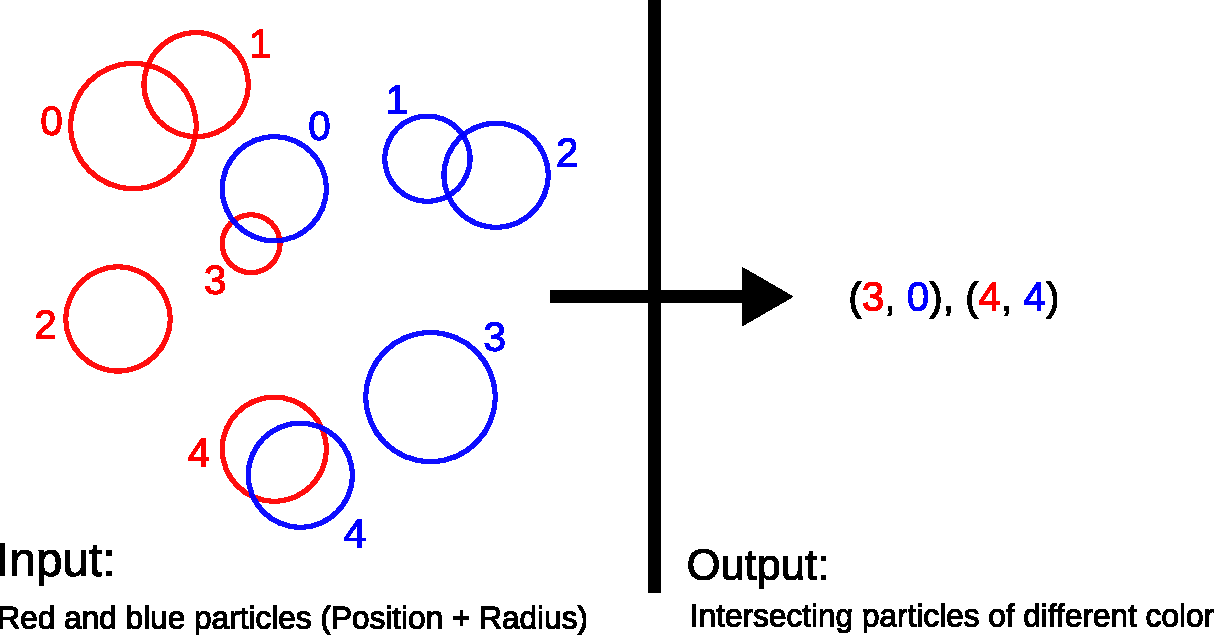
\includegraphics[width=0.7\textwidth]{red_blue_particles}
	\end{figure}
}


\begin{frame}[fragile]
\frametitle{Example: Red-Blue Collision Detection}
\begin{minipage}{0.4\linewidth}
	\vspace{0.3cm}
		\begin{figure}
	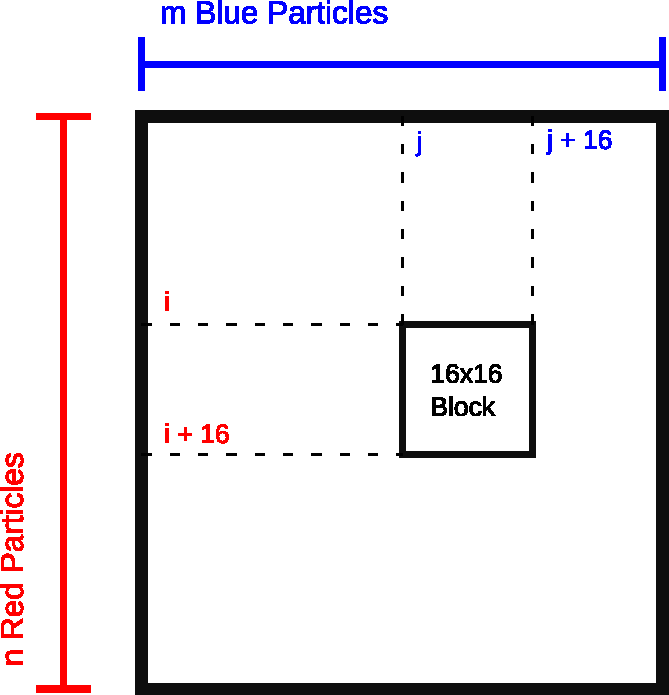
\includegraphics[height=0.7\textheight]{red_blue_particles2}
\end{figure}
\end{minipage}
\begin{minipage}{0.57\linewidth}
\begin{enumerate}
	\item Launch a 2 dimensional grid of threads
	\item Thread $(i,j)$ tests the particle $i$ and $j$
	\item If collision $\rightarrow$ append $(i,j)$ to global list
\end{enumerate}
\end{minipage}
\end{frame}

\begin{frame}[fragile]
\begin{lstlisting}
__global__ void RBPC(Particle* particles1, Particle* particles2, int n, int m, int2* list, int* counter)
{
    int i = blockIdx.x * blockDim.x + threadIdx.x;
    int j = blockIdx.y * blockDim.y + threadIdx.y;
    if (i >= n || j >= m) return;

    const Particle& p1 = particles1[i];
    const Particle& p2 = particles2[j];
    if (Collide(p1, p2))
    {
        int index = atomicAdd(counter, 1);
        if (index < MAX_COLLISIONS)
        {
            list[index] = {i, j};
        }
    }
}
\end{lstlisting}
\end{frame}



\begin{frame}[fragile]
\frametitle{Shared Memory}

Shared Memory (SMEM) is...
\begin{itemize}
	\item located inside the SM
	\item accessible from all threads within a block
	\item very fast (100x) compared to global memory
\end{itemize}
SMEM is typically used for...
\begin{itemize}
	\item communication between threads within a block
	\item caching global memory
\end{itemize}
\end{frame}




\begin{frame}[fragile]
\frametitle{Example: Red-Blue Collision Detection + SMEM}
Idea:
\begin{itemize}
	\item So far, each particle is loaded $n$ times from global memory
	\item[$\rightarrow$] Improve performance by caching the particles in SMEM
\end{itemize}
Implementation (one block):
\begin{enumerate}
	\item Load k red particles and k blue particles to shared memory
	\item Test all $k^2$ intersections and write output
\end{enumerate}
\end{frame}

\begin{frame}[fragile]
\frametitle{Shared Memory (Statically Allocated)}
\begin{itemize}
	\item Created by adding the \texttt{\_\_shared\_\_} keyword to a local variable
	\item Usually used in combination with templating the block size
\end{itemize}
\begin{lstlisting}
template <int BLOCK_SIZE_X, int BLOCK_SIZE_Y, int K>
__global__ void RBPC(Particle* ps1, Particle* ps2, int n, int m)
{
    __shared__ Particle shared_ps1[BLOCK_SIZE_X * K];
    __shared__ Particle shared_ps2[BLOCK_SIZE_Y * K];
    // ...
    shared_ps1[local_offset_i] = ps1[global_offset_i];
    shared_ps2[local_offset_j] = ps2[global_offset_j];
    __syncthreads();
    // ...
}
\end{lstlisting}
\end{frame}




\frame{
	\frametitle{Red-Blue Collision Detection Results}


	\begin{tabular}{l|r}
	Name & Time \\	
	\hline
	GTX 2080 TI  & 0.304 ms\\
	GTX 2080 TI + SMEM  & 0.127 ms\\
	i9-7940X (1 Thread) & 8360 ms \\
	i9-7940X (28 Threads) & 384.1 ms \\
\end{tabular}\textbf{}
\\ \vspace{1cm}

Full Code: \url{https://github.com/darglein/CudaTutorial/blob/master/2_Hardware_and_Communication/Code/collision_detection.cu}
}

\frame{
	\frametitle{Literature}
	%
	\begin{itemize}
		\item \href{https://docs.nvidia.com/cuda/}{CUDA Toolkit Documentation}
		\item \href{https://docs.nvidia.com/gameworks/content/developertools/desktop/analysis/report/cudaexperiments/kernellevel/memorystatisticsglobal.htm}{Global Loads}
		\item \href{https://docs.nvidia.com/cuda/thrust/index.html}{Thrust}
		\item \href{https://github.com/darglein/saiga}{Saiga}
		\item \href{http://developer.download.nvidia.com/CUDA/training/register_spilling.pdf}{Local Memory - Talk}
	\end{itemize}
	
}





\end{document}



